\documentclass[lettersize,journal]{IEEEtran}
\usepackage{graphicx}
\usepackage{amsmath,amsfonts}
\usepackage{algorithm}
\usepackage{algpseudocode}
\usepackage{array}
\usepackage[caption=false,font=normalsize,labelfont=sf,textfont=sf]{subfig}
\usepackage{textcomp}
\usepackage{stfloats}
\usepackage{url}
\usepackage{verbatim}
\usepackage{cite}
\hyphenation{op-tical net-works semi-conduc-tor IEEE-Xplore}
% updated with editorial comments 8/9/2021

\begin{document}

\title{Enhancing Mutual Information Neural Estimation: Theoretical Insights and Practical Applications}

\author{Li Ge \\2022533011}

% The paper headers
\markboth{School of Information Science and Technology, ShanghaiTech University}%
{}

\maketitle

\begin{abstract}
Mutual Information Neural Estimation (MINE) introduces a scalable and trainable neural network-based method for estimating mutual information (MI) with strong consistency. This paper addresses numerical challenges in MI estimation, such as instability from logarithmic and exponential terms, by designing alternative loss functions, including EMA-based smoothing, Softplus, and Log-Sum-Exp, which enhance training stability and convergence.
We further apply MINE in enhancing mode coverage in Generative Adversarial Networks (GANs). Experiments demonstrate that MI regularization accelerates GAN convergence, improving mode diversity.
\end{abstract}

\begin{IEEEkeywords}
Mutual Information, Neural Estimation, Numerical Challenges, GANs, Mode Collapse
\end{IEEEkeywords}

\section{Introduction}
\IEEEPARstart{M}{utual} information (MI) is a key concept in information theory that measures the dependence between variables, capturing non-linear relationships beyond traditional correlation metrics. Its applications include data compression, feature selection, and representation learning.

Accurately estimating MI is challenging, especially for continuous and high-dimensional data. Traditional methods like binning, kernel density estimation (KDE), and likelihood ratio estimators are computationally expensive and require extensive tuning. Recent advances using dual formulations of divergences, such as the Kullback-Leibler (KL) divergence, and adversarial methods have shown promise but are often task-specific and constrained.

The Mutual Information Neural Estimator (MINE) addresses these challenges by providing a scalable, trainable framework for MI estimation based on the dual KL-divergence representation. Key advantages include:
\begin{itemize}
    \item Linear scalability with data dimension and size.
    \item Theoretical consistency guarantees.
    \item Flexibility for MI maximization and minimization tasks.
\end{itemize}

This paper extends MINE by proposing novel loss functions to improve training stability and convergence and test MINE's effect on enhancing mode coverage in GANs using MI regularization.
These contributions advance both the theoretical foundations and practical applications of MINE in generative modeling and representation learning.

The paper is structured as follows: Section II provides a detailed analysis of MINE. Section III, IV, V presents our own experiment based on MINE. Finally, Section VI concludes with key findings and future directions.

\section{MINE Analysis}

\subsection{Background}
\subsubsection{Mutual Information}
Mutual Information (MI) quantifies the statistical dependency between two random variables. It is defined as:
\begin{equation}
    I(X; Z) = D_{KL}(P_{XZ} || P_X \otimes P_Z),
\end{equation}
where $D_{KL}(\cdot || \cdot)$ represents the Kullback-Leibler (KL) divergence, $P_{XZ}$ is the joint distribution, and $P_X \otimes P_Z$ is the product of the marginal distributions. Intuitively, MI measures how much knowing one variable reduces uncertainty about the other. If $X$ and $Z$ are independent, $I(X; Z) = 0$.

\subsubsection{Donsker-Varadhan Representation}
The KL divergence can be expressed as:
\begin{equation}
    D_{KL}(P || Q) = \sup_{T: \Omega \to \mathbb{R}} \mathbb{E}_P[T] - \log \mathbb{E}_Q[e^T],
\end{equation}
where the supremum is taken over all measurable functions $T$ that satisfy integrability constraints. This representation provides a foundation for training neural networks to estimate MI.

\subsubsection{f-Divergence Representation}
An alternative representation is given by:
\begin{equation}
    D_{KL}(P || Q) \geq \sup_{T \in \mathcal{F}} \mathbb{E}_P[T] - \mathbb{E}_Q[e^{T-1}],
\end{equation}
where $\mathcal{F}$ is a class of functions. Although computationally efficient, this method offers a looser bound compared to the Donsker-Varadhan representation.


\subsection{The Mutual Information Neural Estimator (MINE)}
\subsubsection{Core Idea}
MINE utilizes neural networks to parametrize the function \( T_\theta \) in the Donsker-Varadhan representation of the Kullback-Leibler (KL) divergence. This approach enables an efficient and scalable estimation of mutual information (MI) through gradient-based optimization.

\subsubsection{Mathematical Formulation}
The Donsker-Varadhan representation of the KL divergence is given by:
\begin{equation}
D_{\text{KL}}(P \| Q) = \sup_{T} \mathbb{E}_P[T] - \log \mathbb{E}_Q\left[e^T\right],
\end{equation}
where the supremum is taken over all functions \( T \) such that the expectations are finite.

Using this representation, MI can be expressed as:
\begin{equation}
I(X; Z) = \sup_{\theta \in \Theta} \mathbb{E}_{P_{XZ}}[T_\theta] - \log \mathbb{E}_{P_X \otimes P_Z}\left[e^{T_\theta}\right],
\end{equation}
where \( T_\theta \) is a function parametrized by a neural network, \( \Theta \) is the parameter space, and \( P_X \otimes P_Z \) denotes the product of the marginal distributions.

\subsection{Implementation Details}
\subsubsection{Statistics Network}
The function \( T_\theta(X, Z) \) is parameterized by a deep neural network, often a multilayer perceptron (MLP). The input is the paired variables \( (X, Z) \), and the output is a scalar value. Non-linear activation functions such as ReLU or Leaky ReLU are commonly used in the hidden layers.

\subsubsection{Training Procedure}
To estimate MI, MINE optimizes the following objective:
\begin{equation}
\mathcal{L} = -\mathbb{E}_{P_{XZ}}[T_\theta] + \log \mathbb{E}_{P_X \otimes P_Z}\left[e^{T_\theta}\right].
\end{equation}
The training involves the following steps:
\begin{enumerate}
    \item Sample mini-batches from the joint distribution \( P_{XZ} \) and the marginal distribution \( P_X \otimes P_Z \).
    \item Compute \( T = T_\theta(X, Z) \) and \( e^T = e^{T_\theta(X', Z')} \), where \( (X', Z') \) are sampled from \( P_X \otimes P_Z \).
    \item Update an exponential moving average (EMA) for \( e^T \) to reduce bias:
    \begin{equation}
    \text{EMA}(e^T) = (1 - \alpha) \cdot \text{EMA}_{\text{prev}}(e^T) + \alpha \cdot \text{mean}(e^T).
    \end{equation}
    \item To improve numerical stability and convergence, update network parameters \( \theta \) by minimizing the loss:
    \begin{equation}
    \mathcal{L} = -\mathbb{E}_{P_{XZ}}[T_\theta] + \log \text{EMA}(e^T).
    \end{equation}
\end{enumerate}

\subsection{Theoretical Properties}
\subsubsection{Consistency}
MINE ensures that the estimated MI converges to the true MI as the sample size increases. This property is guaranteed by:

\textbf{The universal approximation theorem}: ensures \( T_\theta \) can approximate any continuous function given sufficient network capacity.

\textbf{Classical consistency theorems for extremum estimators}: confirm that MI estimates improve with more samples.

\subsubsection{Sample Complexity}
The sample complexity of MINE is given by:
\begin{equation}
\tilde{O}\left(\frac{d \log d}{\epsilon^2}\right),
\end{equation}
where \( d \) is the dimension of the parameter space and \( \epsilon \) is the desired error.

\subsection{Experiments from the Original MINE Paper}
This section analyzes the three key experimental applications presented in the original MINE paper, which demonstrate its versatility across various machine learning tasks.

\subsubsection{Mode-Dropping in Generative Adversarial Networks (GANs)}
Mode collapse is a common issue in GANs, where the generator fails to produce diverse samples, leading to underrepresentation of certain modes in the data distribution.

\textbf{Approach:} A mutual information regularization term is added to the generator's loss function, encouraging diverse samples by maximizing the mutual information between generated samples and input noise variables.

\textbf{Experiment Results:} 
Adding MINE-based regularization significantly improved mode coverage for both Spiral and 25-Gaussians datasets. Visual comparisons showed that the generator uniformly covered all modes without mode-dropping.

\textbf{Analysis:} 
This experiment demonstrates MINE's capability to enhance mode diversity in GANs, a critical feature for generating realistic and diverse outputs.

\subsubsection{Reconstruction in Adversarially Learned Inference (ALI)}
Adversarially Learned Inference (ALI) often lacks fidelity in data reconstruction since its training objective matches the joint distributions of data and latent variables without directly optimizing reconstruction error.

\textbf{Metrics:} Reconstruction quality is evaluated using:
\begin{enumerate}
    \item Euclidean reconstruction error.
    \item Reconstruction accuracy, defined as the proportion of labels preserved by the reconstructed samples using a pre-trained classifier.
    \item Multi-scale Structural Similarity Index (MS-SSIM), assessing perceptual quality.
\end{enumerate}

\textbf{Datasets:} Increasingly complex datasets, including 25-Gaussians, MNIST, and CelebA.

\textbf{Approach:} MINE maximizes the mutual information between latent representations and reconstructed data to reduce reconstruction error.

\textbf{Results:}
MINE achieved significantly lower reconstruction errors compared to ALI. 
While ALICE (a variation of ALI) performed slightly better in reconstruction, it suffered from mode-dropping, which MINE effectively addressed.

\textbf{Analysis:} 
MINE improves reconstruction fidelity while maintaining robust mode representation in adversarial inference models.

\subsubsection{Information Bottleneck in a Continuous Setting}
The Information Bottleneck (IB) framework extracts relevant information from an input \(X\) to predict an output \(Y\), but is challenging to apply in continuous settings due to the intractability of computing mutual information.

\textbf{Dataset:} Permutation-invariant MNIST, where pixel positions are randomly permuted, removing spatial dependencies.

\textbf{Encoders:} Three types of encoders were evaluated:
\begin{enumerate}
    \item Gaussian encoder: \( z = \mu(x) + \sigma \epsilon, \epsilon \sim \mathcal{N}(0, I) \).
    \item Additive noise encoder: \( z = \text{enc}(x + \sigma \epsilon), \epsilon \sim \mathcal{N}(0, I) \).
    \item Propagated noise encoder: \( z = \text{enc}([x, \epsilon]), \epsilon \sim \mathcal{N}(0, I) \).
\end{enumerate}

\textbf{Comparison:} MINE was compared to the Deep Variational Bottleneck (DVB), which relies on variational bounds to estimate mutual information.

\textbf{Results:}
MINE outperformed DVB in terms of misclassification rates across all encoder types.
Unlike DVB, MINE does not require tractable density assumptions, making it more robust and versatile.

\textbf{Analysis:}
This experiment demonstrates MINE's advantage in continuous IB applications, achieving superior performance and flexibility compared to traditional methods.

\subsubsection{Conclusion}
The original MINE experiments successfully showcased its strengths in:
\begin{itemize}
    \item Enhancing mode diversity in GANs.
    \item Improving reconstruction fidelity in adversarial inference models.
    \item Enabling robust applications of Information Bottleneck in continuous settings.
\end{itemize}
These results lay the foundation for our further exploration and experiments.

\section{Experiment 1: on 3-D Gaussian and 4-D Gaussian}
This experiment focuses on the original MINE and aims to test how well the MINE network can estimate the mutual information and the effect of different loss functions on estimating mutual information.
\subsection{Experimental Setup}
To ensure a rigorous evaluation, we designed our experiments with the following setup:

\textbf{Dataset:} For MI estimation, we utilized multivariate Gaussian distributions. Specifically, 3-dimensional and 4-dimensional Gaussian distributions with standardized normal marginals were chosen due to their analytically computable MI using the correlation coefficient $\rho$:
    \[
    I(X; Z) = -\frac{1}{2} \log(1 - \rho^2).
    \]
    
\textbf{Statistics Network:} We implemented a fully connected neural network as the statistics network \( T_\theta \), consisting of three hidden layers with 128 units each, employing the LeakyReLU activation function.
    
\textbf{Optimization:} For training, we adopted the Adam optimizer with an initial learning rate of $1 \times 10^{-3}$, decayed over time to accelerate convergence. Gradient clipping was applied to avoid instability caused by large gradients.
    
\textbf{Loss Function Variants:} Besides the original loss function, we explored alternative designs, including:
    \begin{enumerate}
        \item \textbf{Exponential Moving Average (EMA) Loss:} Smoothens gradient updates using an EMA of the marginal mean, improving stability.
        \item \textbf{Softplus Loss:} Replaces the log function with a smooth approximation, enhancing numerical stability.
        \item \textbf{Clipped Gradient Loss:} Limits gradient magnitude to mitigate instability at the cost of potential bias.
        \item \textbf{Log-Sum-Exp Loss:} Prevents numerical overflow while considering contributions from sparse data.
        \item \textbf{Regularized Loss:} Adds a penalty term to prevent overfitting and improve generalization.
        \item \textbf{Noise-Augmented Loss:} Introduces Gaussian noise to encourage robustness and exploration.
    \end{enumerate}
    
\textbf{Evaluation Metrics:} The primary metric for MI estimation accuracy was the root-mean-square error (RMSE) between the estimated MI and the ground truth. For generative modeling, we visually inspected the mode coverage and convergence speed.

This standardized setup ensured consistency across all experiments while allowing us to focus on the comparative analysis of different loss functions and their impact on MINE's performance.

\subsection{Experiment Results}
In this section, we present and analyze the visual and quantitative results of mutual information (MI) estimation for 3D and 4D Gaussian datasets. The visualizations include generated samples, MI estimates over epochs, and comparative performance of different loss functions.

\subsubsection{Generated Samples for 3D and 4D Gaussians}
Figure~\ref{fig:gaussian_samples} shows the generated samples for 3D and 4D Gaussian datasets. The samples were drawn from the distributions estimated using the statistics network trained with the original and modified loss functions.

\begin{figure}[h]
    \centering
    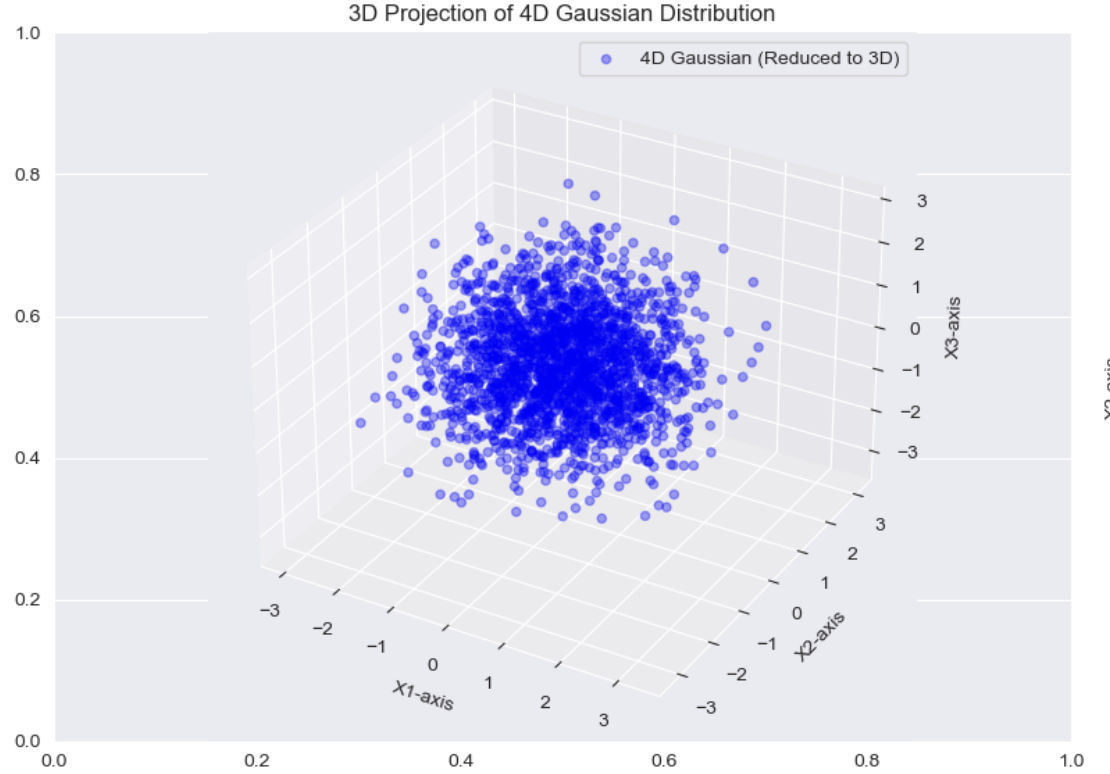
\includegraphics[width=0.45\linewidth]{figures/4d_gaussian_samples_1.png}
    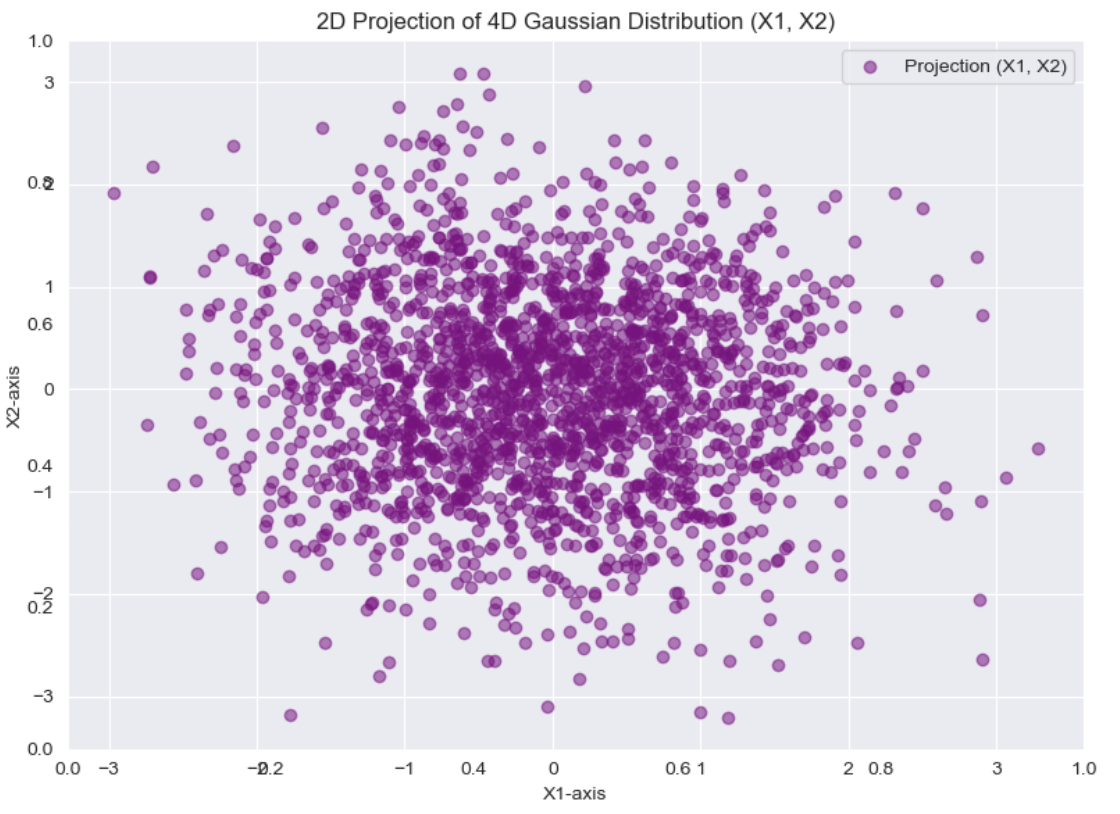
\includegraphics[width=0.45\linewidth]{figures/4d_gaussian_samples_2.png}
    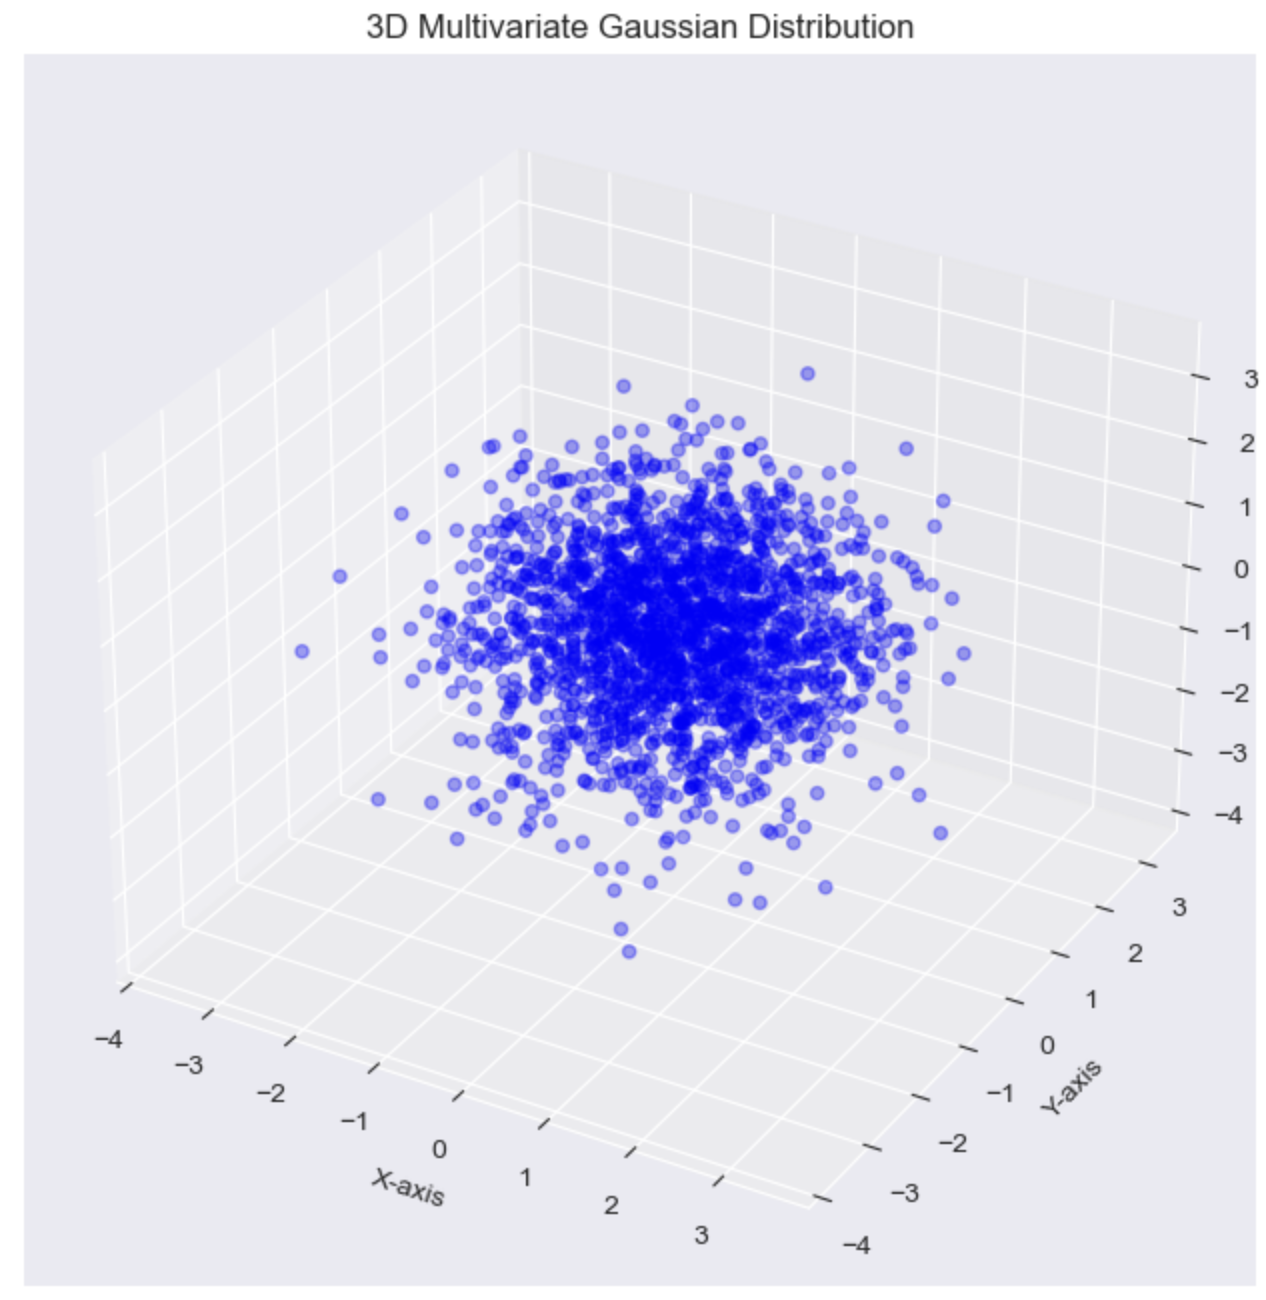
\includegraphics[width=0.45\linewidth]{figures/3d_gaussian_samples.png}
    \caption{Generated samples for 3D (below) Gaussian and 4D (above, right one is the 3-d projection, left one is the 2-d projection of the first two dimensions) Gaussian datasets using the MINE network. Different loss functions demonstrate varying levels of stability and alignment with the true distribution.}
    \label{fig:gaussian_samples}
\end{figure}

\subsubsection{Mutual Information Estimation Over Epochs}
The MI estimation for 3D and 4D Gaussian datasets is presented in Figure~\ref{fig:mi_estimates}. Key observation is that the estimated MI here is unstable.

\begin{figure}[h]
    \centering
    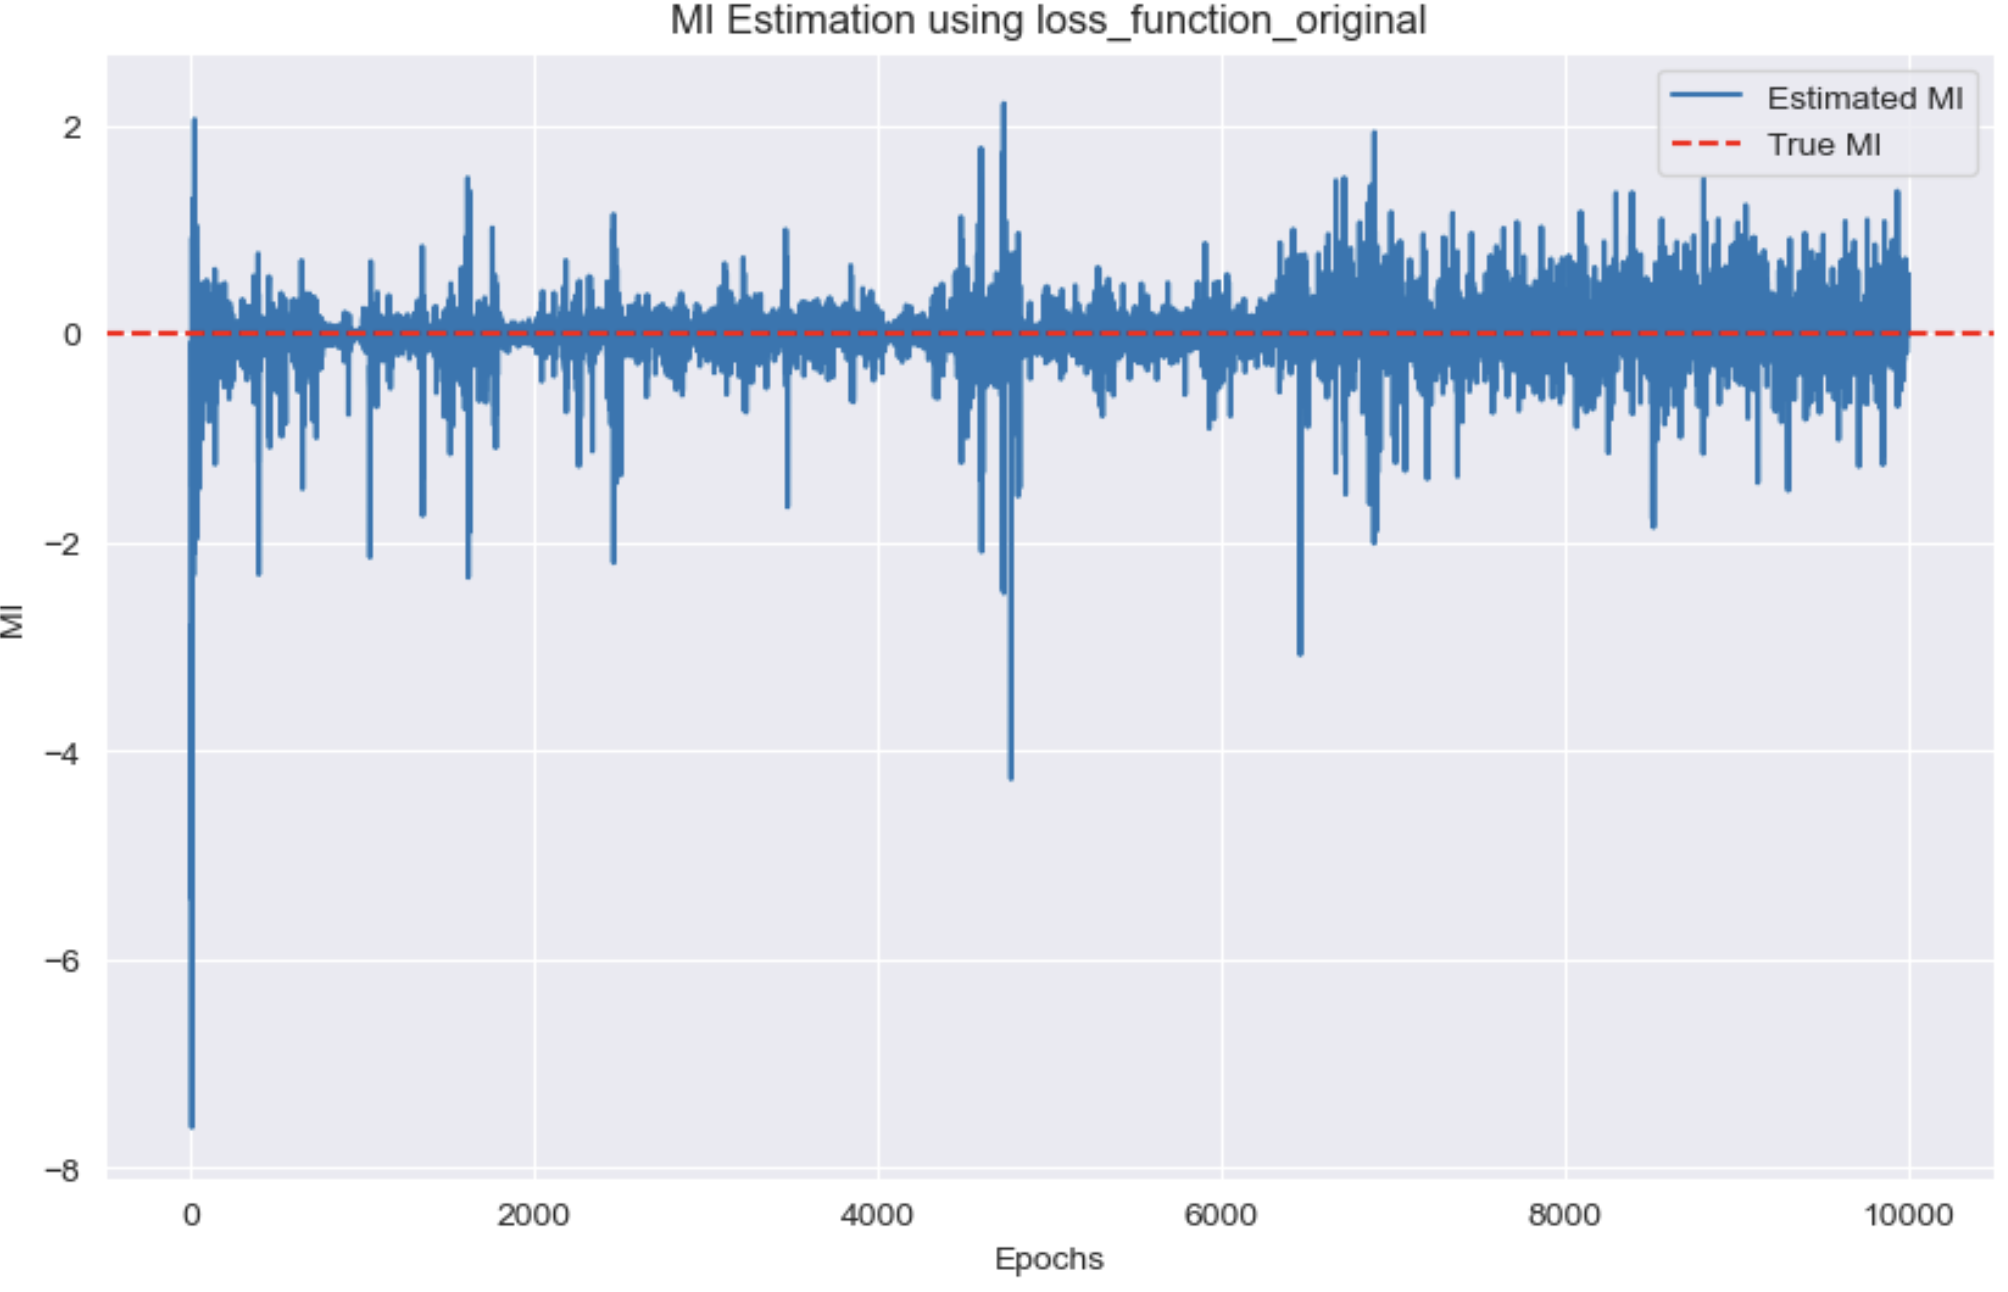
\includegraphics[width=1\linewidth]{figures/3d_mi_estimates.png}
    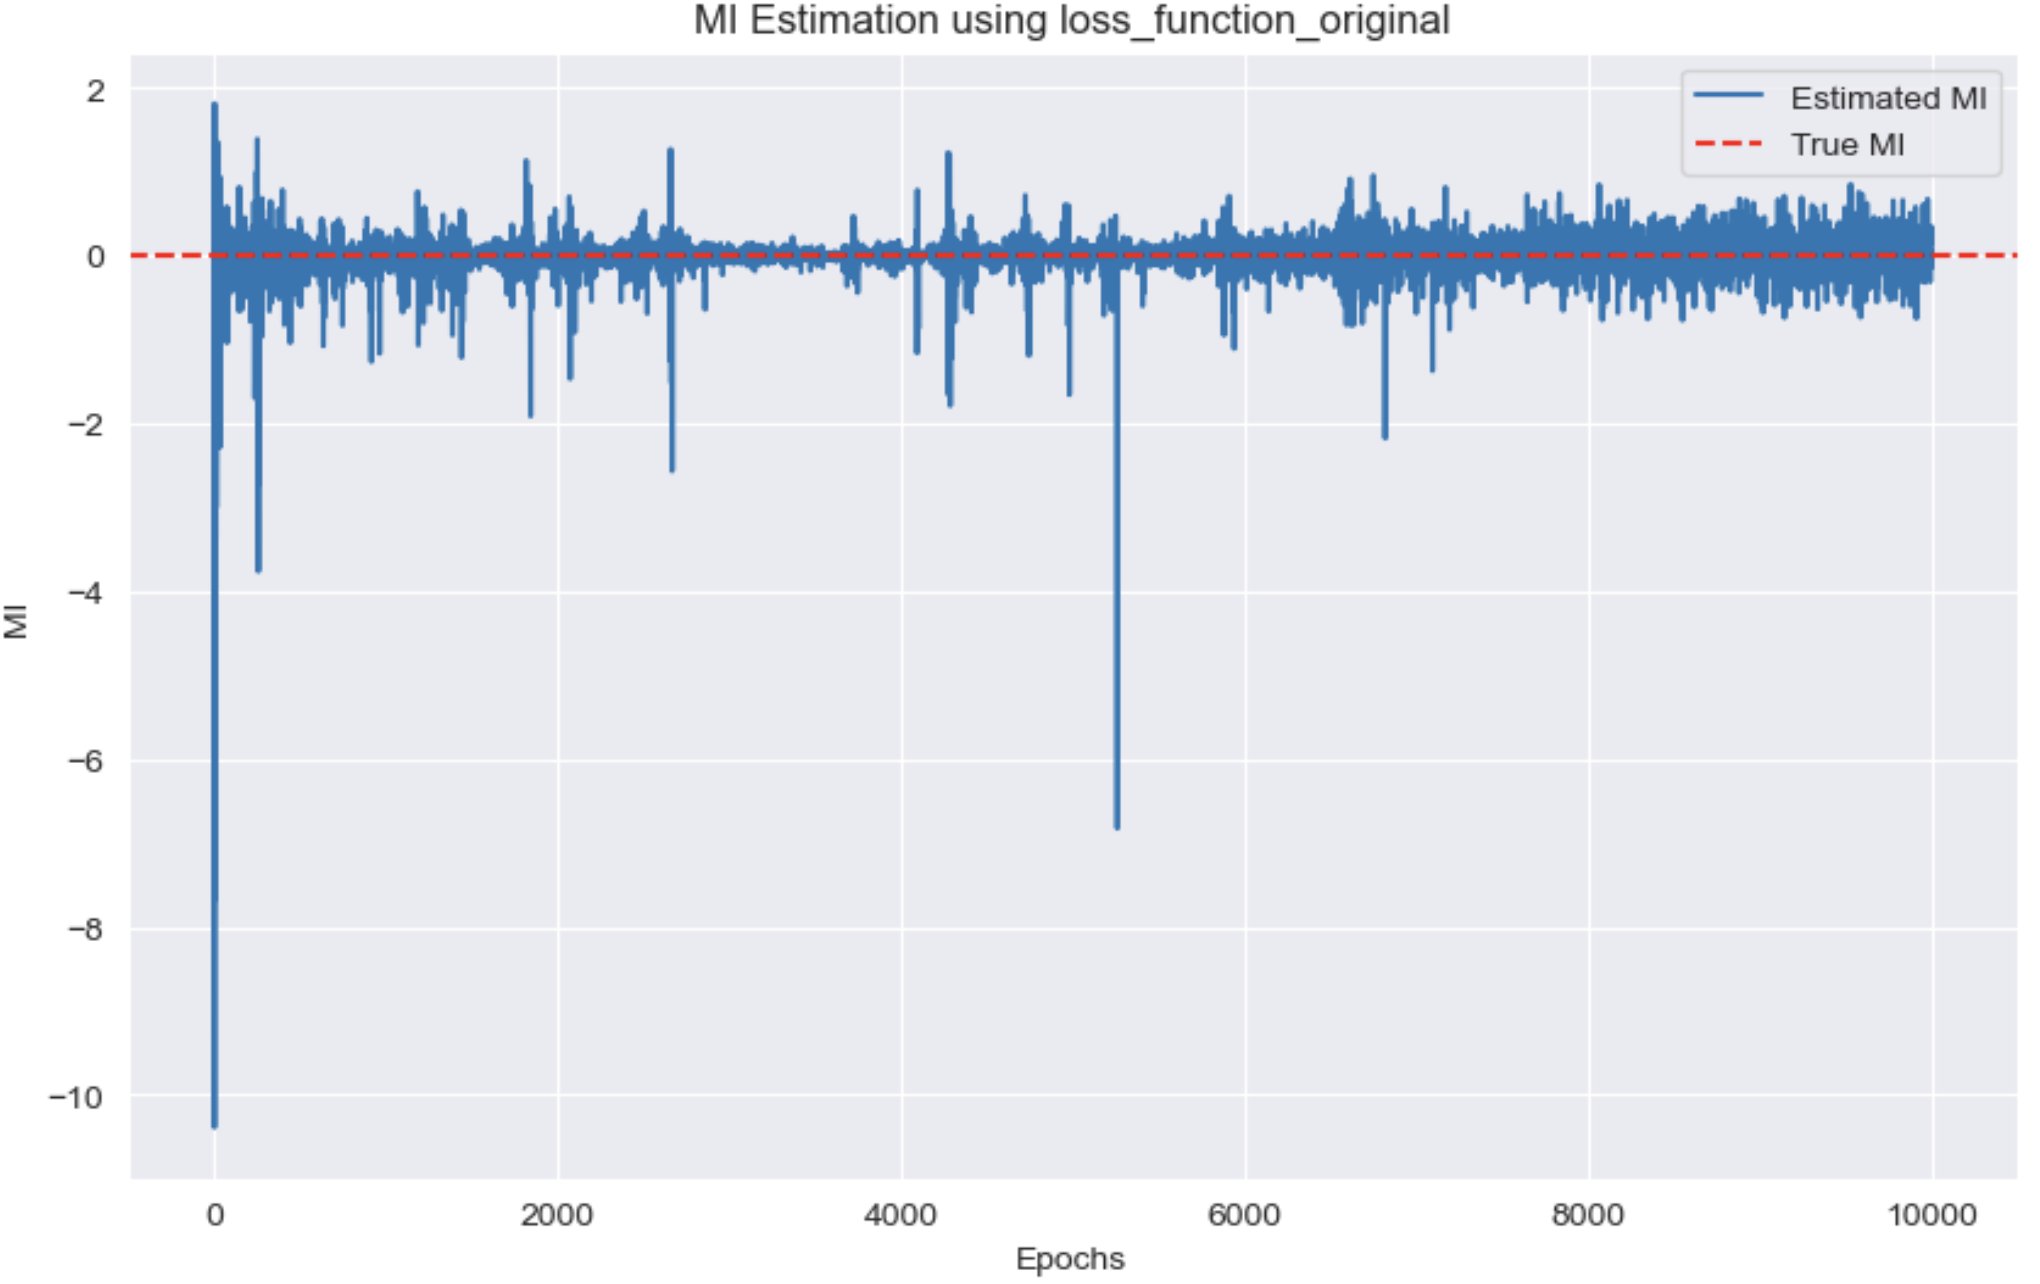
\includegraphics[width=1\linewidth]{figures/4d_mi_estimates.png}
    \caption{Estimated MI during training for (left) 3D Gaussian and (right) 4D Gaussian datasets using original loss function. The ground truth MI is indicated by a dashed line.}
    \label{fig:mi_estimates}
\end{figure}

\subsubsection{Performance Across Loss Functions}
Figure~\ref{fig:loss_comparisons} compares the MI estimation performance across the six proposed loss functions. Each plot represents the deviation of the estimated MI from the ground truth for both datasets:
\begin{itemize}
    \item \textbf{Log-Sum-Exp Loss:} Demonstrated the smallest deviation for both datasets, validating its numerical stability and robustness against high-dimensional complexity.
    \item \textbf{Regularized Loss:} Achieved similar performance to log-sum-exp, particularly for 3D data, but required careful tuning of EMA parameters.
    \item \textbf{Softplus Loss:} Provided stable performance but with a slight approximation bias, leading to marginally higher deviations.
    \item \textbf{Clipped Gradient and Noise-Augmented Losses:} Both showed larger deviations, particularly for 4D data, indicating challenges in stability and convergence.
\end{itemize}

\begin{figure}[h]
    \centering
    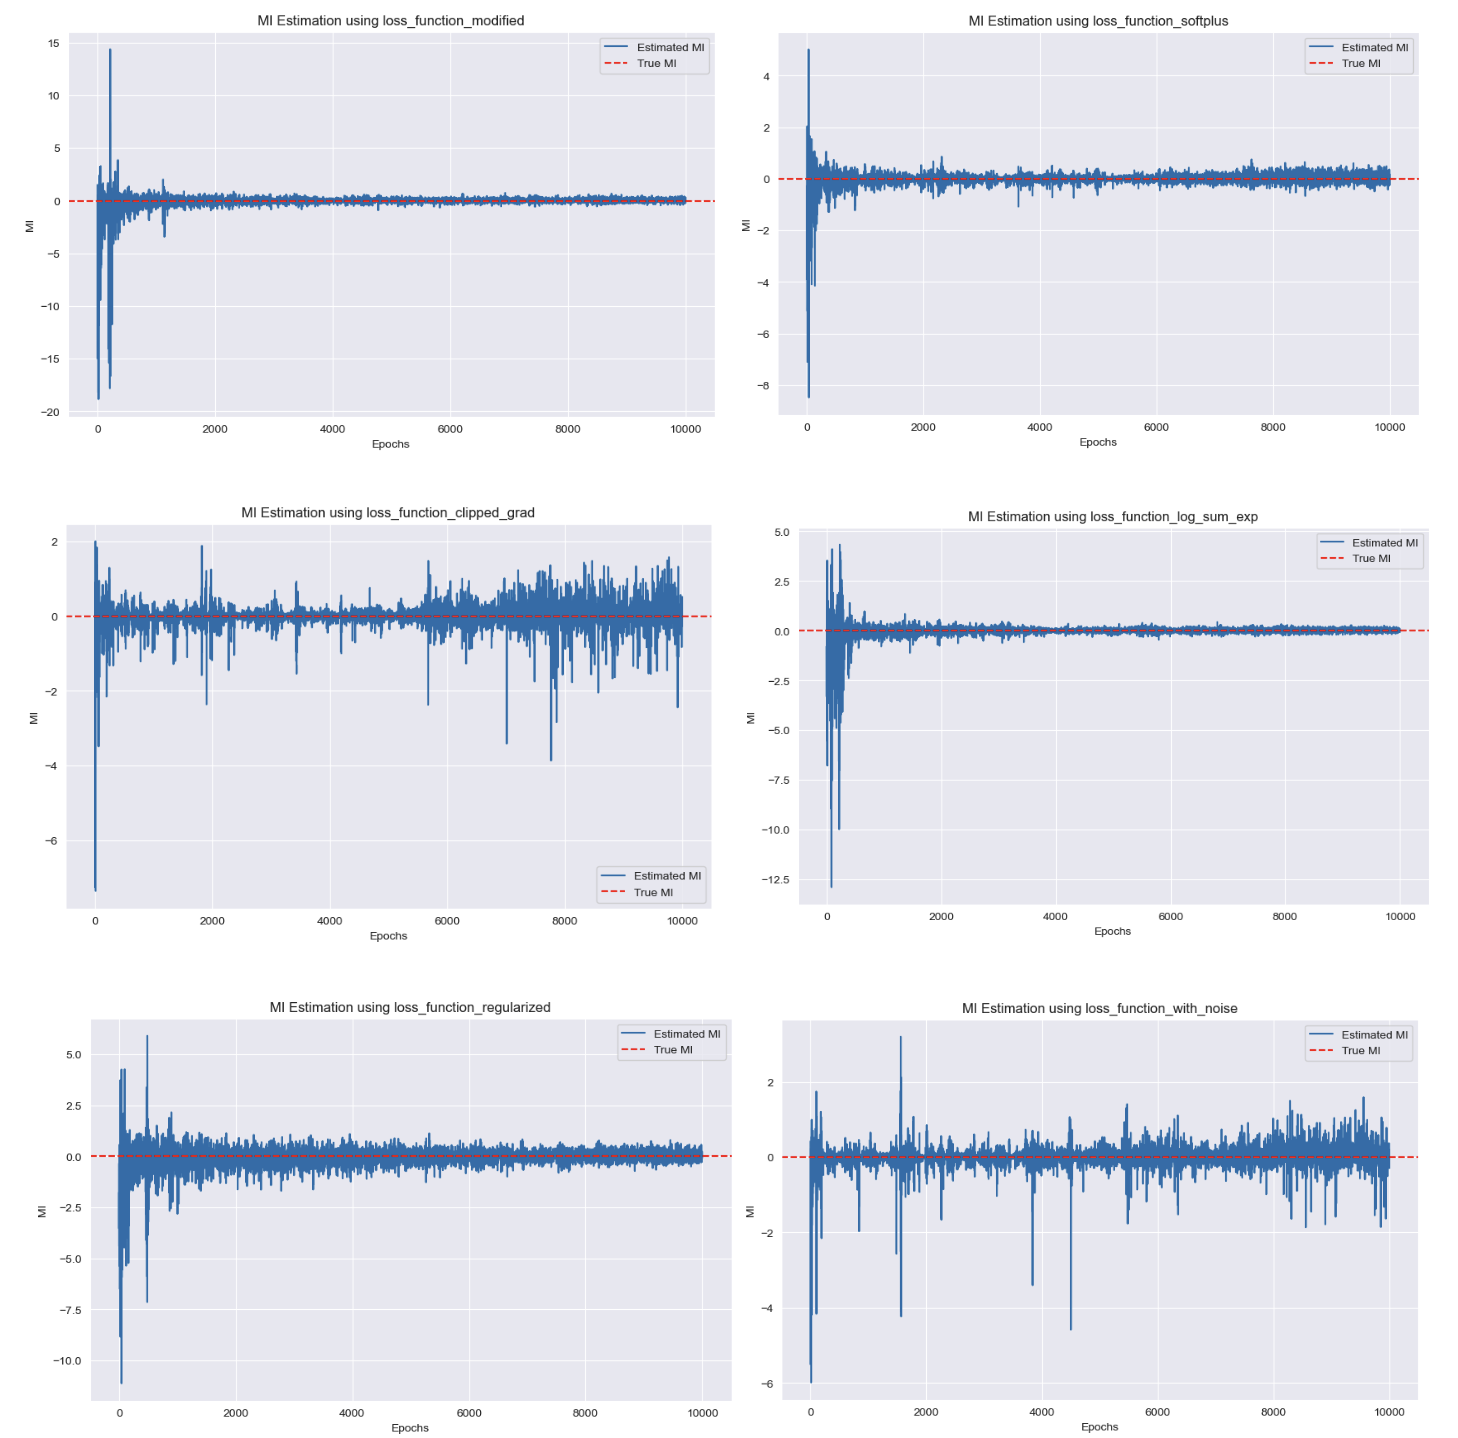
\includegraphics[width=1\linewidth]{figures/3d_loss_comparisons.png}
    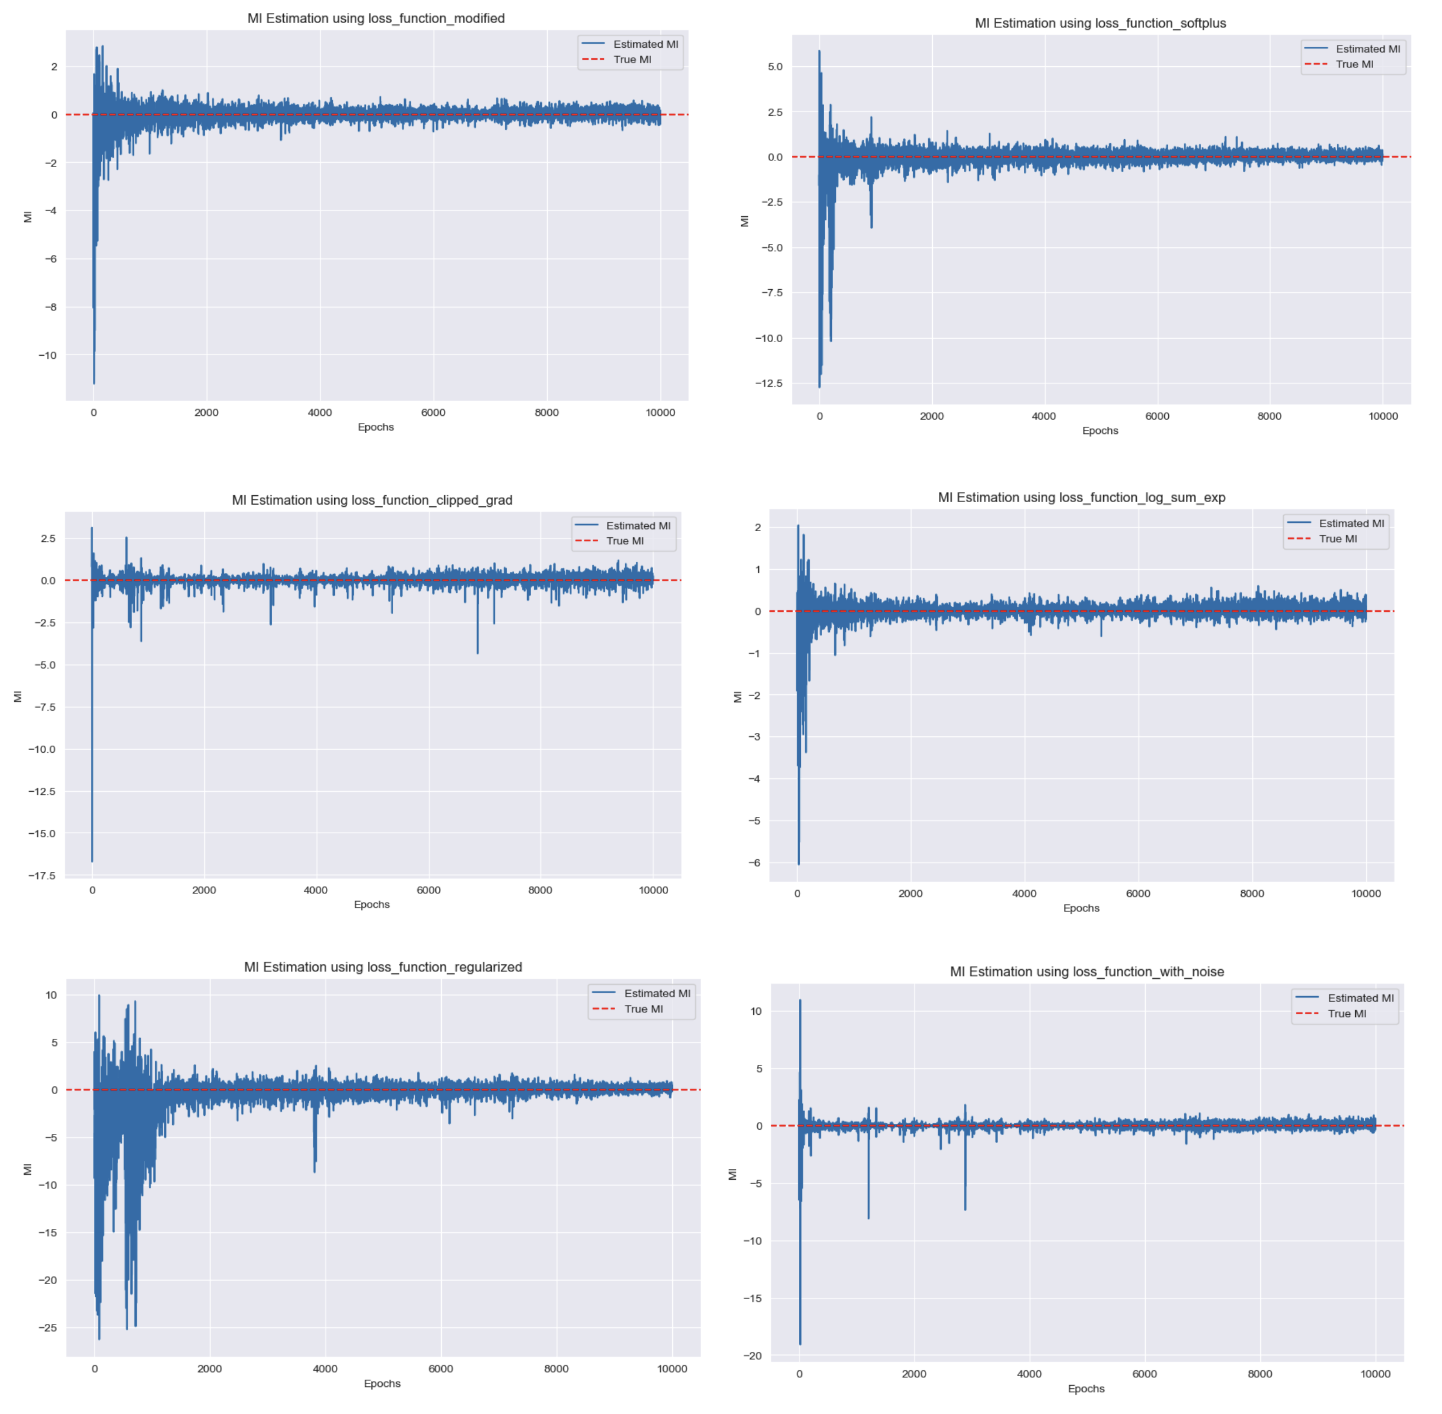
\includegraphics[width=1\linewidth]{figures/4d_loss_comparisons.png}
    \caption{Comparison of MI estimation deviations across six loss functions for (six figures above) 3D Gaussian and (six figures below) 4D Gaussian datasets. Log-sum-exp and EMA losses consistently outperform others.}
    \label{fig:loss_comparisons}
\end{figure}


    \textbf{Exponential Moving Average (EMA) Loss:} 
    $$\mathcal L = - \left( \mathbb{E}_{P(X, Z)}[t] - \frac{1}{\mathbb{E}[\text{ma}(e^{t})]}\cdot \mathbb{E}_{P(X)P(Z)}\left[e^{t}\right] \right)$$
    This loss exhibited stable convergence across both 3D and 4D Gaussian datasets. By smoothing the gradient updates, the loss reduced oscillations during training, leading to significantly smaller RMSE compared to the original loss.
    \begin{itemize}
        \item \textit{Strengths:} Smooths gradient updates, reduces noise sensitivity, and prevents extreme oscillations in training.
        \item \textit{Weaknesses:} Requires careful tuning of the EMA parameter, which can impact convergence speed.
    \end{itemize}
    
    \textbf{Softplus Loss:}
  $$\mathcal{L} = - \left( \mathbb{E}_{P(X, Z)}[t] - \text{Softplus}\left(\mathbb{E}_{P(X)P(Z)}[e^t]\right) \right)$$
  The softplus approximation effectively avoided numerical issues caused by extreme values in the log function. While its RMSE was slightly higher than EMA, it provided consistent convergence behavior without significant spikes.
    \begin{itemize}
        \item \textit{Strengths:} Provides a smooth approximation to the log function, enhancing numerical stability.
        \item \textit{Weaknesses:} Introduces approximation bias, which may limit accuracy in scenarios requiring high precision.
    \end{itemize}
    
    \textbf{Clipped Gradient Loss:} 
  $$\mathcal{L} = - \left( \mathbb{E}_{P(X, Z)}[t] - \log \mathbb{E}_{P(X)P(Z)}[e^t] \right)$$
  This loss mitigated gradient explosion by bounding gradient magnitudes. However, the clipping introduced bias in gradient updates, resulting in slower convergence and suboptimal accuracy.
    \begin{itemize}
        \item \textit{Strengths:} Prevents gradient explosion, particularly useful for noisy datasets.
        \item \textit{Weaknesses:} Modifies the true gradient direction, leading to suboptimal convergence and instability.
    \end{itemize}
    
    \textbf{Log-Sum-Exp Loss:} 
  $$\mathcal{L} = - \left( \mathbb{E}_{P(X, Z)}[t] - \log \sum_{i} e^{t_i - \max(t)} \right)$$
  Log-sum-exp yielded the best RMSE, demonstrating exceptional stability. By leveraging the maximum term in the summation, it prevented numerical overflow while still considering contributions from smaller terms.
    \begin{itemize}
        \item \textit{Strengths:} Prevents numerical overflow/underflow, ensures stability, and provides tight approximations to the true MI.
        \item \textit{Weaknesses:} Computationally more expensive due to summation over all terms.
    \end{itemize}
    
    \textbf{Regularized Loss:} 
  $$\mathcal{L} = - \left( \mathbb{E}_{P(X, Z)}[t] - \log \mathbb{E}_{P(X)P(Z)}[e^t] \right) + \lambda \|e^t\|_2^2$$
  The addition of a regularization term improved generalization. While convergence was slower, the estimator was more robust to overfitting, particularly on higher-dimensional datasets.
    \begin{itemize}
        \item \textit{Strengths:} Reduces overfitting and improves generalization by penalizing large magnitudes of \( e^t \).
        \item \textit{Weaknesses:} Requires additional hyperparameter tuning for the regularization coefficient \( \lambda \).
    \end{itemize}
    
    \textbf{Noise-Augmented Loss:} 
  $$\mathcal {L} = - \left( \mathbb{E}_{P(X, Z)}[t + \mathcal{N}(0, \sigma^2)] - \log \mathbb{E}_{P(X)P(Z)}[e^t] \right)$$
  Introducing Gaussian noise improved robustness but added instability during optimization. This instability was pronounced on higher-dimensional datasets, resulting in less consistent MI estimates.
    \begin{itemize}
        \item \textit{Strengths:} Encourages exploration and improves robustness by regularizing the optimization landscape.
        \item \textit{Weaknesses:} Adds randomness to optimization, potentially slowing convergence and causing instability.
    \end{itemize}

\subsubsection{Concluding Observations}
The experimental results demonstrate that MINE's performance heavily depends on the choice of loss function. While log-sum-exp and regularized loss functions provided the best stability, others like noise-augmented or clipped gradient losses faced challenges in convergence and accuracy.

\section{Experiment 2: Circular Dataset}
The circular dataset experiment was designed to evaluate the performance of MINE in improving mode coverage and accelerating convergence in generative adversarial networks (GANs). 

The new loss of the generator is:
$$\arg \max_G E[log(D(G([\epsilon, c])))] + \beta I(G([\epsilon, c]); c)$$
where $\beta I(G([\epsilon, c]); c)$ is the mutual information regularization term. In this experiment and the next experiment, we aim to explore its effect.

\subsection{Experiment Setup}
We designed our experiments with the following setup:

\textbf{Dataset:} The circular dataset is defined as points uniformly sampled along a 2D circle of radius \( r = 5 \). Noise is added to each point by sampling from a Gaussian distribution \( \mathcal{N}(0, 0.1^2) \), creating a slightly perturbed circular pattern. The dataset contains 10,000 samples, split into 80\% training and 20\% testing sets.
\begin{figure}[h]
    \centering
    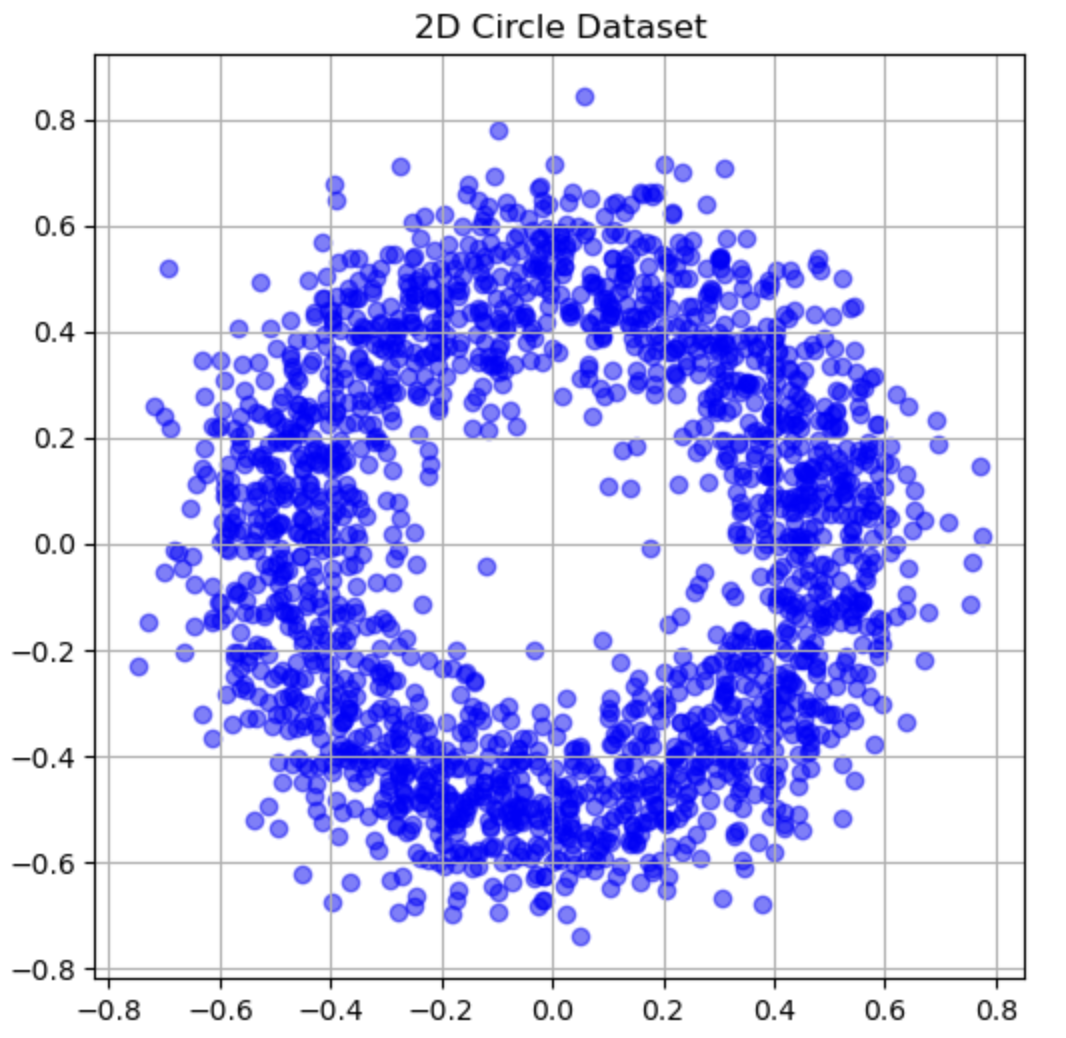
\includegraphics[width=0.55\linewidth]{figures/circular_samples.png}
    \caption{Original circular samples.}
    \label{fig:original_samples}
\end{figure}
    
    \textbf{Model Architecture:}
    Apart from the regular networks (generator and discriminator), we added another statistical network (MINE) to output the estimated mutual information.
    
    \textbf{Loss Functions:}
    \begin{itemize}
        \item GAN Loss: We used the Wasserstein GAN (WGAN) loss with gradient penalty for stable training.
        \item MI Regularization: The mutual information estimated by MINE is added to the generator's loss function with a weighting coefficient \( \beta \).
    \end{itemize}
    
    \textbf{Experimental Variants:} Different values of \( \beta \) (0, 1, 0.1, 0.01, 0.001) were tested to understand the impact of MI regularization strength. A baseline GAN without MI regularization (\( \beta = 0 \)) served as the control experiment.
    
    \textbf{Evaluation Metrics:}
    Mode Coverage (the ability of the generator to represent all regions of the circular distribution) an convergence Speed (the number of epochs required for the generator to produce stable and complete samples).
    
    \textbf{Training Details:} The model was trained for 20 epochs with a batch size of 128. The Adam optimizer was used with a learning rate of \( 10^{-3} \) for all networks. The learning rate was decayed using a cosine schedule to improve convergence.

\subsection{Results and Analysis}

The results of the circular dataset experiment demonstrate the impact of incorporating MINE-based mutual information (MI) regularization on GAN performance. This section presents the experimental observations and provides a detailed analysis of the outcomes.

\subsubsection{Generated Sample Quality}
Figure~\ref{fig:circular_samples} shows the generated samples at different epochs for various regularization weights (\( \beta \)). Key observations include:

    \textbf{Baseline GAN (\( \beta = 0 \)):} Without MI regularization, the generator begins to produce stable samples that cover the circular distribution after approximately 8 epochs. However, mode collapse is evident in earlier epochs, with the generator focusing on specific segments of the circle.
    
    \textbf{With MI Regularization (\( \beta = 1, 0.1, 0.01, 0.001 \)):} Adding MI regularization significantly accelerates convergence. Stable and complete coverage of the circular distribution is achieved within the first 2 epochs for all nonzero \( \beta \) values, demonstrating the effectiveness of MI in guiding the generator towards better mode representation.

\subsubsection{Convergence Speed}
Table~\ref{tab:circular_convergence} summarizes the convergence speed (measured in epochs) for different regularization weights. The results indicate:

The convergence speed improves as \( \beta \) increases from \( 0.001 \) to \( 0.1 \), showing that stronger regularization enhances training dynamics.

For \( \beta = 1 \), the generator's performance is less stable, with noisy samples observed even after 6 epochs, suggesting over-regularization.
\begin{table}[h]
    \centering
    \begin{tabular}{c|c}
        \hline
        \textbf{Regularization Weight \( \beta \)} & \textbf{Convergence Speed (Epochs)} \\
        \hline
        0 & 8 \\
        0.001 & 2 \\
        0.01 & 2 \\
        0.1 & 2 \\
        1 & 2 \\
        \hline
    \end{tabular}
    \caption{Convergence speed for different \( \beta \) values. Convergence is defined as stable and complete mode coverage.}
    \label{tab:circular_convergence}
\end{table}

\subsubsection{Analysis of Regularization Weight \( \beta \)}
The experiments highlight the importance of selecting an appropriate \( \beta \) value:
\begin{itemize}
    \item Small values of \( \beta \) (e.g., \( 0.001 \)) provide mild regularization, improving stability without significantly affecting convergence speed.
    \item Moderate values (e.g., \( 0.1 \)) achieve the best balance, leading to rapid convergence and stable mode coverage.
    \item Large values (e.g., \( 1 \)) result in over-regularization, where the generator excessively focuses on MI optimization, neglecting other aspects of the GAN objective.
\end{itemize}

\subsubsection{Implications and Insights}

The results demonstrate that MI plays a critical role in stabilizing GAN training and improving mode coverage. When MI stabilizes, the generated samples also converge to the target distribution.

The oscillations in MI for \( \beta = 1 \) highlight the challenges of over-regularization, where excessive focus on MI can hinder the generator's ability to balance the GAN objectives.

The relationship between MI and sample stability underscores the potential of MINE-based regularization to enhance GAN training across various datasets and distributions.

\begin{figure}[h]
    \centering
    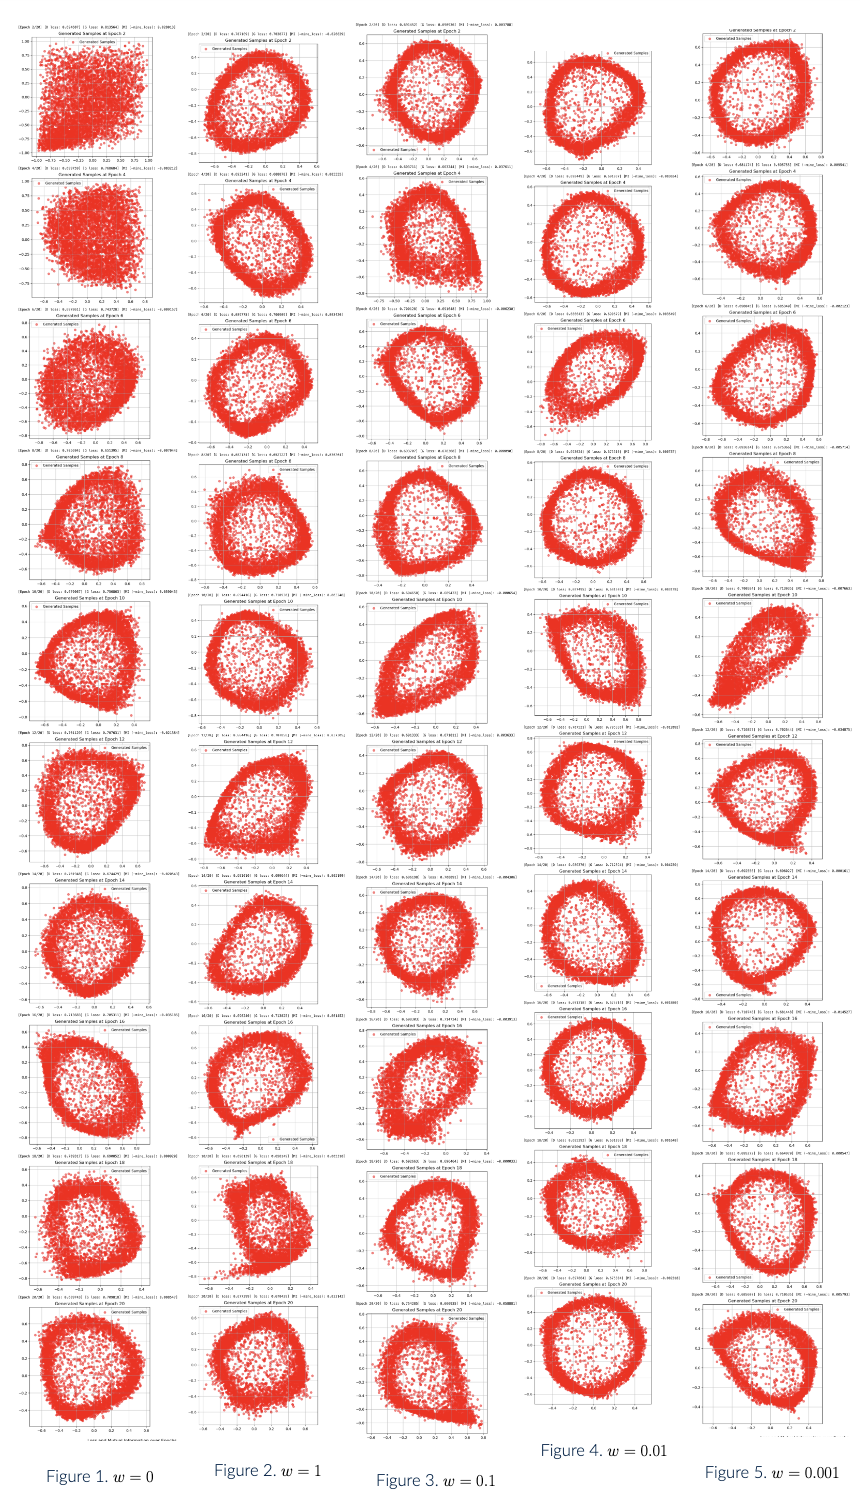
\includegraphics[width=1\linewidth]{figures/gg.png}
    \caption{Generated samples for different regularization weights (\( \omega \)) at various epochs. Here we use \( \omega \) to represent the MI coefficient \( \beta \) mentioned above.}
    \label{fig:circular_samples}
\end{figure}

\section{Experiment 3: Cross-Shaped Dataset}
\subsection{Experiment Setup}

This experiment investigates the performance of MINE-regularized GANs on a more complex cross-shaped data distribution. The primary goal is to evaluate how effectively the mutual information (MI) regularization term improves mode coverage and accelerates training stability, particularly under varying regularization strengths.

\subsubsection{Dataset and GAN Configuration}
We designed a synthetic cross-shaped dataset, characterized by two intersecting lines forming a "+" shape in two-dimensional space. This distribution is more challenging than the circular dataset, requiring the generator to learn and represent multiple disjoint regions simultaneously. The GAN architecture, including the generator \( G \), discriminator \( D \), and MINE network \( M \), was identical to the previous experiment.

\subsubsection{Regularization Coefficients}
We explored five different regularization strengths (\( \beta \)): 0 (no MI regularization), 1, 0.1, 0.01, and 0.001. The coefficient \( \beta \) controls the weight of the MI term in the generator loss function, balancing the focus between sample fidelity and mutual information.

\subsubsection{Training Strategy}
Given the increased complexity of the cross-shaped dataset, the GAN required more training epochs for convergence:
Initially, the epoch limit was set to 100, with output visualizations every 10 epochs.
For more efficient evaluation, we adjusted the maximum epochs to 10, recording the generator output after each epoch.

\subsection{Experiment Results}

The results of the cross-shaped dataset experiment highlight the impact of mutual information (MI) regularization on GAN training, particularly for challenging multi-modal distributions. Below, we present detailed analyses of the generated samples, convergence behavior, and mutual information estimates.

\subsubsection{Visualization of Generated Samples}  
Figure \ref{fig:cross-distribution} shows the original cross-shaped dataset, which consists of two intersecting lines in 2D space. Figures \ref{fig:100-epochs} and \ref{fig:10-epochs} compare the generated distributions under different regularization weights \( \beta \).

\begin{figure}[!ht]
    \centering
    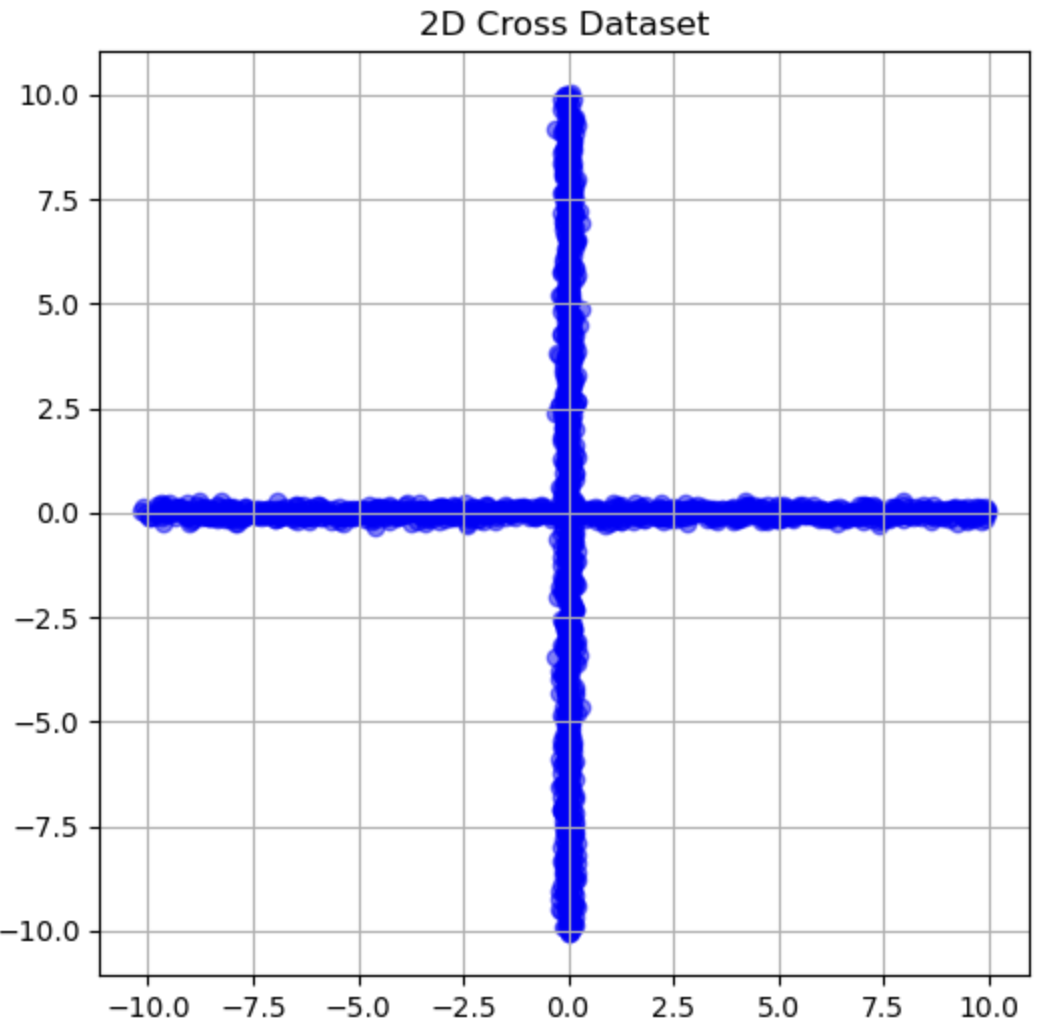
\includegraphics[width=0.55\linewidth]{figures/cross_original.png}
    \caption{Original Cross-shaped Distribution}
    \label{fig:cross-distribution}
\end{figure}

\begin{figure}[!ht]
    \centering
    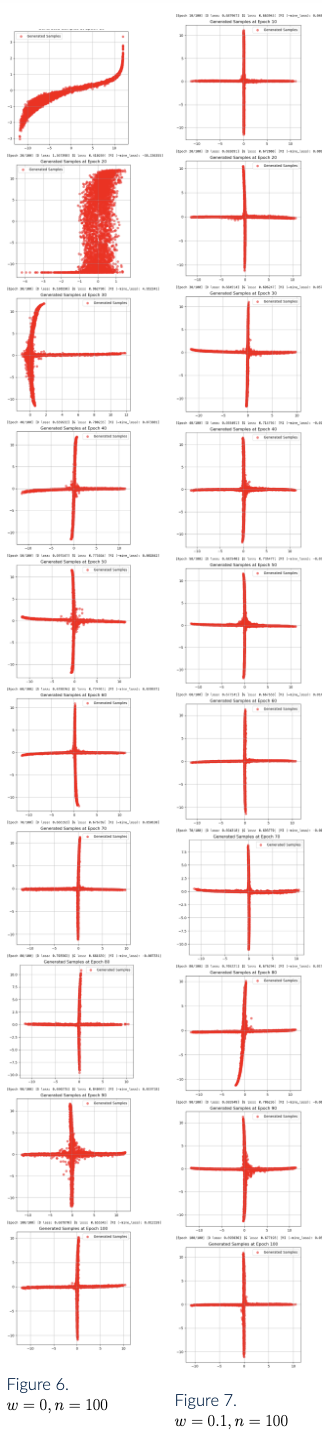
\includegraphics[width=0.5\linewidth]{figures/cross_100epochs.png}
    \caption{Comparison of Generated Samples at 100 Epochs (Left: \( \beta = 0 \), Right: \( \beta = 0.1 \))}
    \label{fig:100-epochs}
\end{figure}

\begin{figure}[!ht]
    \centering
    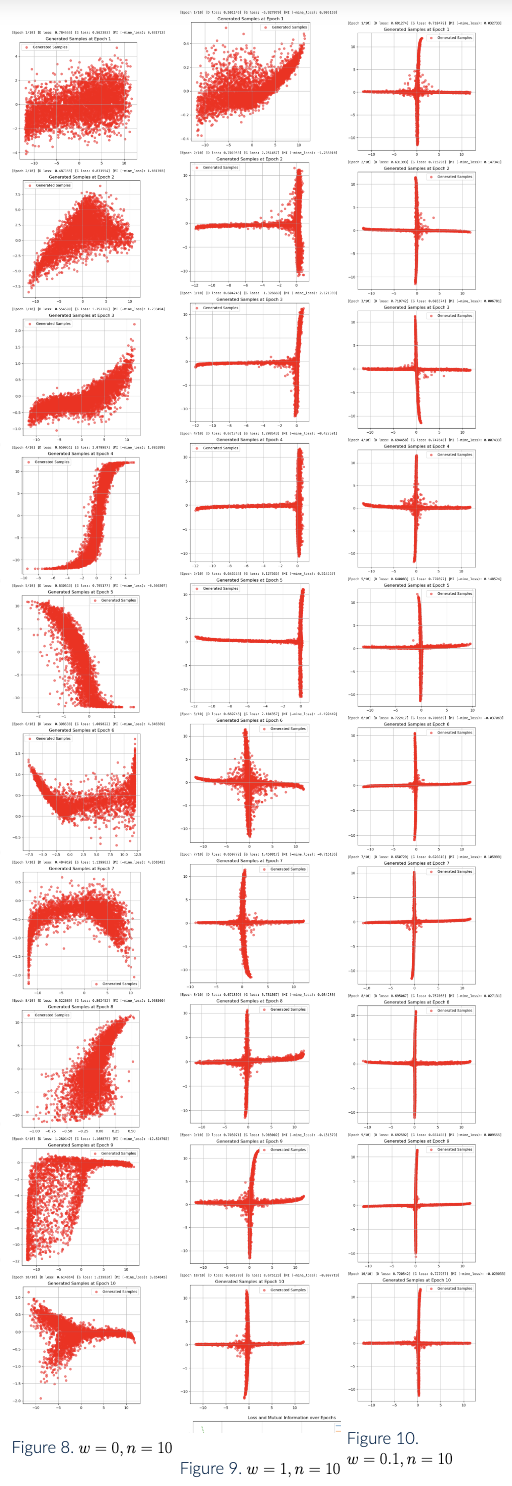
\includegraphics[width=0.5\linewidth]{figures/cross_10epochs.png}
    \caption{Comparison of Generated Samples at 10 Epochs (Left to Right: \( \beta = 0 \), \( \beta = 1 \), \( \beta = 0.1 \))}
    \label{fig:10-epochs}
\end{figure}

The following observations can be made:
1. Without MI regularization (\( \beta = 0 \)), the generator converges slowly, producing incomplete representations of the cross distribution until epoch 40 or later.
2. Moderate regularization strengths (\( \beta = 0.1, 0.01, 0.001 \)) enable rapid convergence, with stable and accurate outputs by epoch 10.
3. Excessive regularization (\( \beta = 1 \)) results in noisy outputs, requiring additional epochs to stabilize, as shown in Figure \ref{fig:10-epochs}.

\subsubsection{Mutual Information Estimates}  
Figures \ref{fig:mi-100epochs} depicts the estimated MI (negative MINE loss) over epochs. This result illustrates the relationship between MI stability and generator performance.

\begin{figure}[!ht]
    \centering
    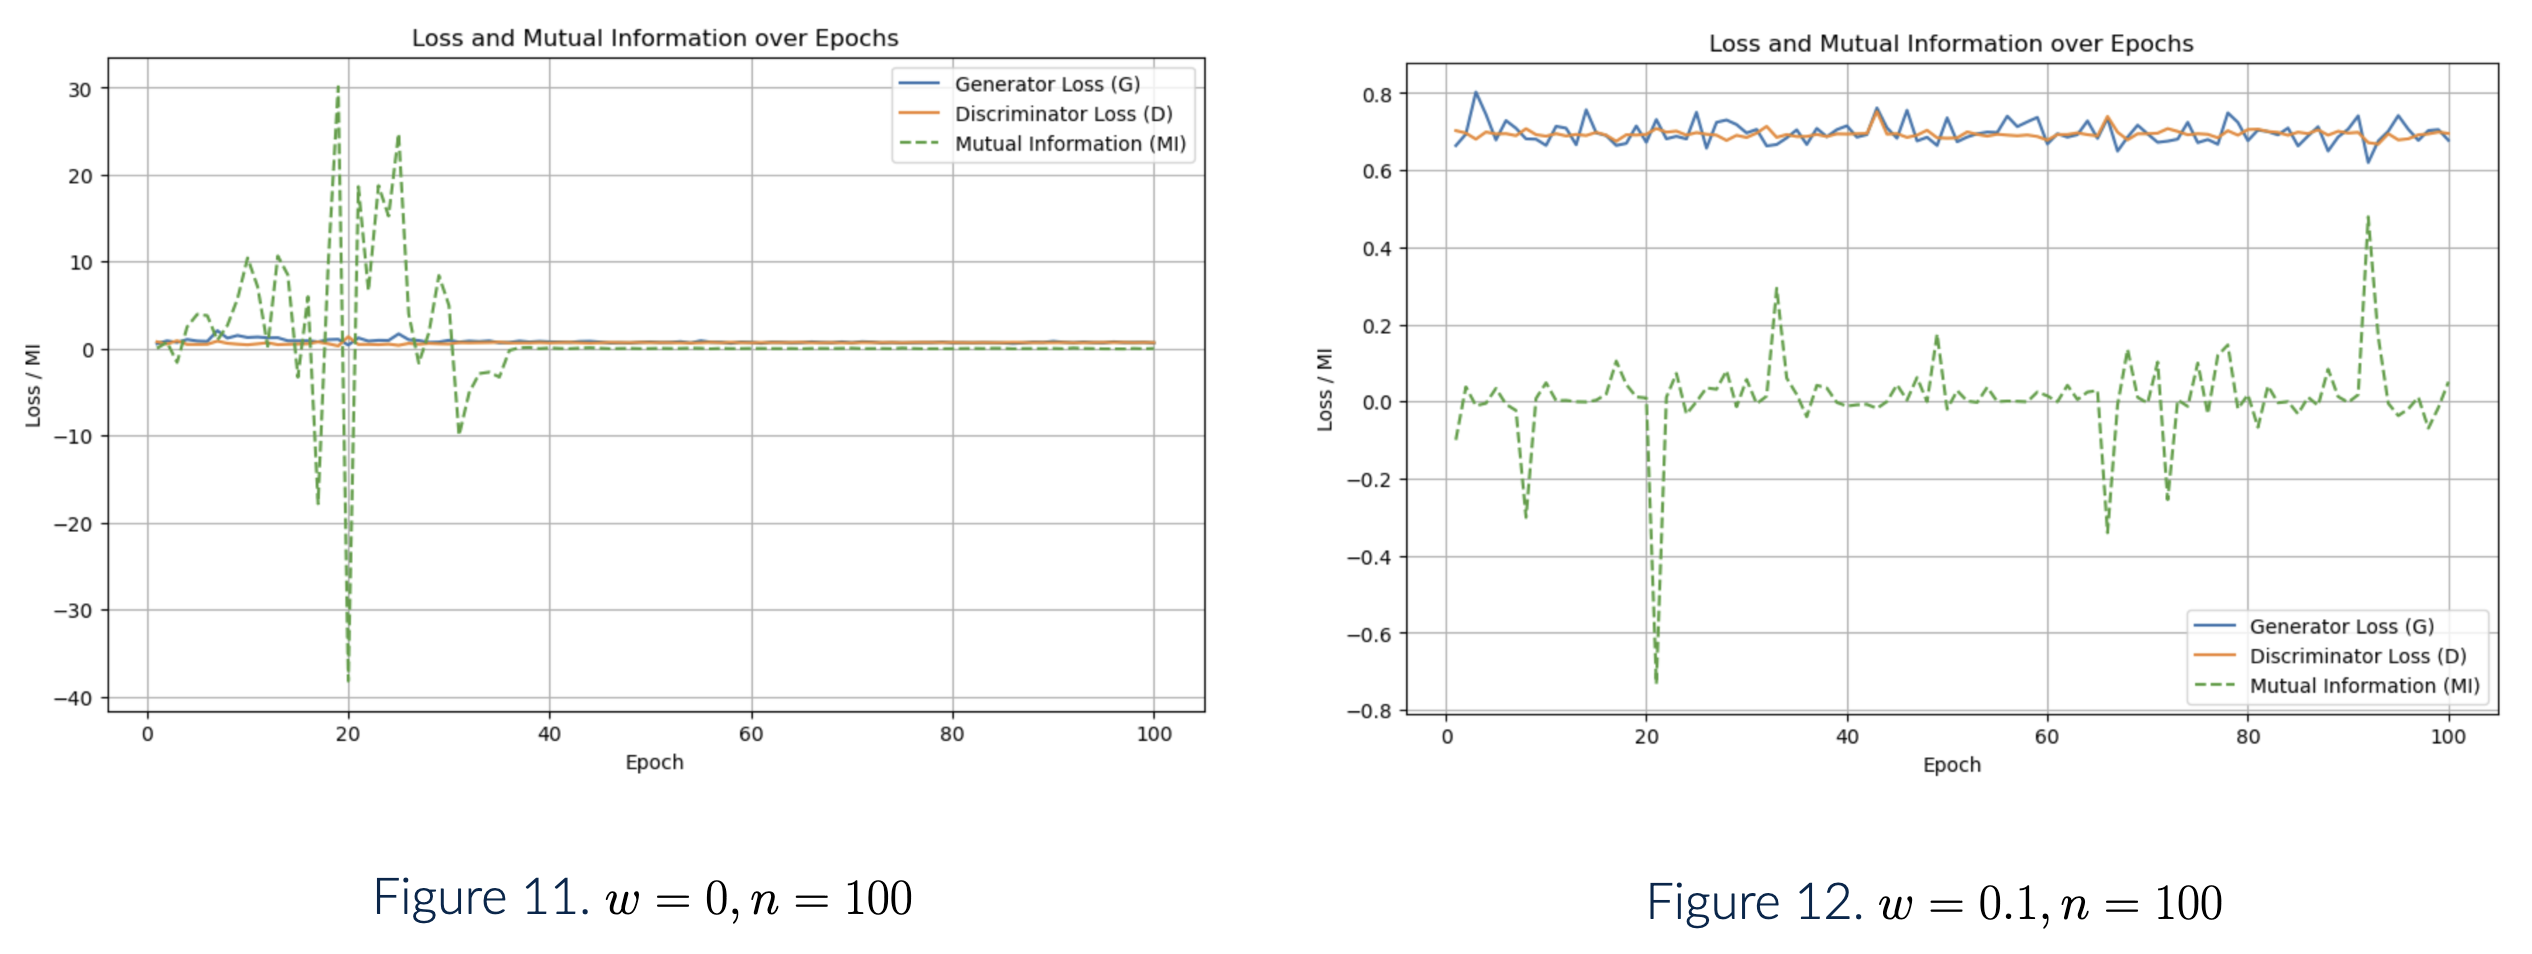
\includegraphics[width=1\linewidth]{figures/mi_100epochs.png}
    \caption{MI Evolution Over 100 Epochs (Left: \( \beta = 0 \), Right: \( \beta = 0.1 \))}
    \label{fig:mi-100epochs}
\end{figure}

Key observations include:
- Without MI regularization, the MI estimate stabilizes only after epoch 40, correlating with the delayed convergence of generated samples.
- With moderate regularization, MI estimates stabilize near-zero as early as epoch 1, ensuring rapid convergence and improved mode coverage.
- Excessive regularization (\( \beta = 1 \)) causes instability in MI estimates, reflecting noisy outputs in generated samples.

\subsubsection{Convergence Observations}
Without MI regularization (\( \beta = 0 \)), the GAN exhibited slow convergence, taking up to 40 epochs to produce stable outputs that covered the cross-shaped distribution adequately.
When MI regularization was applied, convergence was significantly accelerated. Across all \( \beta \) values, the generator produced stable and accurate outputs within 10 epochs.

Notably, for \( \beta = 1 \), the convergence behavior was less consistent, with noisy outputs persisting until epoch 6. Stability and complete mode coverage were only achieved at epoch 7. This suggests that excessive regularization may disrupt the generator's focus on optimizing \( \mathbb{E}[t] \), leading to suboptimal performance.

\subsubsection{Mutual Information Monitoring}
We also tracked the estimated MI (negative MINE loss) during training to analyze its relationship with convergence:

Without regularization, the MI only began stabilizing around epoch 40, aligning with the delayed stabilization of generator outputs.

With regularization, MI estimates stabilized as early as epoch 1, consistent with the rapid convergence of generator outputs. The stabilization of MI at near-zero values further validated MINE's capability to optimize the generator's latent space efficiently.

\subsubsection{Key Insights and Hypotheses}  
Moderate values of \( \beta \) (e.g., 0.1) balance the trade-off between stability and convergence speed. Excessive regularization prioritizes MI optimization at the cost of fidelity, as evidenced by the slower stabilization for \( \beta = 1 \).

\textbf{MI Stability and Mode Coverage:} The synchronization between MI stabilization and mode coverage underscores MI's critical role in guiding GAN convergence. Stable MI values ensure accurate and diverse sample generation.

\textbf{Impact of Regularization:} Excessive MI regularization disrupts the generator's optimization of \( \mathbb{E}[t] \), suggesting the need for balanced loss function design. Future work could explore adaptive weighting strategies to optimize this trade-off.

These findings demonstrate MINE's effectiveness as an MI regularizer, provided the regularization strength is carefully chosen. Further research could refine loss design and explore the broader applicability of MI-based regularization in generative models.

\section{Conclusion}

This paper explored the Mutual Information Neural Estimator (MINE), a scalable neural network-based approach for estimating mutual information (MI). We addressed key challenges in MI estimation, particularly the numerical instability caused by logarithmic and exponential terms, by proposing six alternative loss functions. These include EMA-based smoothing, Softplus, and Log-Sum-Exp, which improved the stability and convergence of MINE.

Through theoretical analysis and extensive experiments, we demonstrated the versatility of MINE:
\begin{itemize}
    \item In MI estimation, MINE achieved accurate and consistent performance on 3D and 4D Gaussian datasets, with significant gains under Log-Sum-Exp and regularized loss modifications.
    \item In generative modeling, MINE-regularized GANs showed improved mode coverage and faster convergence on circular and cross-shaped datasets, particularly with moderate regularization strengths.
\end{itemize}

Our findings highlight MINE's role in enhancing model performance by stabilizing MI estimates, leading to improved convergence and diversity in generative tasks. However, results also underscore the sensitivity to regularization strength, necessitating careful parameter tuning.

In conclusion, this work advances both the theoretical and practical aspects of MINE. By resolving numerical challenges, introducing enhanced loss functions, and demonstrating its effectiveness in various applications, we provide a solid foundation for future research. Potential directions include adaptive regularization, improved network architectures, and integrating MINE into broader frameworks like reinforcement learning and causal inference.


\begin{thebibliography}{1}
\bibliographystyle{IEEEtran}

\bibitem{ref1}
Belghazi, M.I., Baratin, A., Rajeswar, S., Ozair, S., Bengio, Y., Courville, A. and Hjelm, R.D., 2018. Mine: mutual information neural estimation. arXiv preprint arXiv:1801.04062.. American Mathematical Society. [Online]. Available: https://www.ams.org/arc/styleguide/mit-2.pdf

\bibitem{ref2}
Veiner, J., Alajaji, F. and Gharesifard, B., 2024. A unifying generator loss function for generative adversarial networks. Entropy, 26(4), p.290.

\bibitem{ref3}
Zadorozhnyy, V., Cheng, Q. and Ye, Q., 2021. Adaptive weighted discriminator for training generative adversarial networks. In Proceedings of the IEEE/CVF Conference on Computer Vision and Pattern Recognition (pp. 4781-4790).

\end{thebibliography}


\newpage




\vfill

\end{document}


